% =====================================================================
% Why Does My Driving Network Brake Late?
%
% Overleaf: upload or paste this single file and compile with pdfLaTeX
% (the default).  Every figure is drawn with TikZ/pgfplots, so there are
% no image files to upload.  Figures marked "schematic" in their caption
% illustrate a definition; they are not recorded data.
% =====================================================================
\documentclass[conference]{IEEEtran}
\IEEEoverridecommandlockouts

\usepackage{cite}
\usepackage{amsmath,amssymb}
\usepackage{graphicx}
\usepackage{booktabs}
\usepackage{array}
\usepackage{xcolor}
\usepackage{textcomp}
\usepackage{tikz}
\usepackage{pgfplots}
\usetikzlibrary{arrows.meta,positioning,calc,fit,backgrounds}
\usepgfplotslibrary{fillbetween}
\pgfplotsset{compat=1.16}
\usepackage[hidelinks]{hyperref}
\newcolumntype{L}[1]{>{\raggedright\arraybackslash}p{#1}}

\hyphenpenalty=10000
\exhyphenpenalty=10000
\tolerance=9999
\emergencystretch=3em
\sloppy

% ---------------------------------------------------------------------
% Figure style.  Colours are colour-blind safe (Okabe--Ito) and every
% figure also separates its classes by line style or fill, so the
% figures remain readable in a greyscale print.
% ---------------------------------------------------------------------
\definecolor{cObs}{HTML}{0072B2}   % observed by the network
\definecolor{cHid}{HTML}{D55E00}   % hidden / unexplained
\definecolor{cHelp}{HTML}{009E73}  % safety helpers
\definecolor{cInk}{HTML}{333333}

\tikzset{
  box/.style={draw=cInk!70, rounded corners=1.5pt, fill=white, align=center,
              font=\scriptsize, inner sep=3pt, minimum height=0.8cm,
              line width=0.5pt},
  obs/.style={box, draw=cObs, fill=cObs!8},
  hid/.style={box, draw=cHid, fill=cHid!10},
  help/.style={box, draw=cHelp, fill=cHelp!10},
  flow/.style={-{Stealth[length=4pt]}, line width=0.6pt, draw=cInk!80},
  lbl/.style={font=\scriptsize, text=cInk!85, inner sep=1.5pt, align=center},
}
\pgfplotsset{
  every axis/.append style={font=\scriptsize, tick label style={font=\scriptsize},
                            label style={font=\scriptsize},
                            title style={font=\scriptsize\bfseries}, line width=0.5pt},
}

\begin{document}

\title{Why Does My Driving Network Brake Late?\\[4pt]
{\Large Auditing Hidden Causes and Safety-Helper Dependence\\
in Privileged-State Imitation Learning\par}}

\author{
\IEEEauthorblockN{
Medhansh Khattar,\quad
Prashant Kumar Jaglan,\quad
Yash Yadav\\[2pt]
Samyak Jain,\quad
Sanchit Kumar Sinha,\quad
Aryan Garg}
}

\maketitle

% =====================================================================
\begin{abstract}
A network that copies an expert driver can only be as good as the
information it is given. If the expert reacts to something that is
missing from the network's inputs, no amount of training data or tuning
will fix the copy. Reported results rarely check for this. We propose a
simple audit, run before training, that asks whether the expert's
actions can be explained by the inputs at all. We define
\emph{unexplained action events}, such as brake onsets that no input
warns of, and report the share of them as the Unexplained Event Rate
(UER). On a small CARLA imitation dataset (19{,}750 samples, 12 routes)
we found that the expert began braking 40 times while moving and that
35 of those onsets had no warning in any of the network's eight inputs,
a UER of 87.5\% (95\% Wilson interval 73.9--94.5\%). A second
contribution is a three-way evaluation that separates the network's
skill from that of the safety helpers around it. The dataset statistics
in Section~\ref{sec:prelim} are measured. The cause attribution,
feature-repair and helper-attribution experiments are specified as
protocols, and we report no results for them.
\end{abstract}

\begin{IEEEkeywords}
imitation learning, behaviour cloning, partial observability,
observability audit, safety shield, CARLA
\end{IEEEkeywords}

% =====================================================================
\section{Introduction}

Behaviour cloning trains a network to reproduce the actions of an
expert~\cite{bojarski}. The usual report is a low prediction error on
held out data. That number says how well the network copies the expert
\emph{given its inputs}. It does not say whether those inputs contain
what the expert was reacting to.

This matters most when the expert is a program with access to the whole
simulator, while the learner receives a short list of derived values
(Fig.~\ref{fig:overview}).
The expert can then act for reasons the learner cannot observe. The
learner will do the best it can, which usually means reacting after the
effect becomes visible, for example braking only once the car has begun
to slow. We call this problem \emph{hidden cause}.

Our motivating case comes from a small CARLA~\cite{carla} project in
which a network with eight inputs imitates CARLA's \texttt{BasicAgent}.
Test error was low (steering mean absolute error 0.015), yet the network
started its stops late. When we looked at the recorded data, 35 of 40
brake onsets had no warning in any input. The low error and the late
stops are consistent: error is averaged over mostly constant frames,
while the failure is concentrated in a few moments of change.

A second problem sits on top of the first. Real driving prototypes
usually wrap the network in safety helpers, such as a supervisor that
applies the brake and rules that restart a stalled car. When the car
completes a route, it is unclear how much credit belongs to the network.
Shielded learning~\cite{shield} makes the system safe but can also hide
how weak the learned part is.

We make three contributions, all designed to be cheap to run on a
single-machine setup:
\begin{enumerate}
\setlength{\itemsep}{1pt}
\item \textbf{An observability audit.} We define unexplained action
events and the Unexplained Event Rate (UER), and a predictive lead-time
test that can be run before any network is trained (Section~\ref{sec:audit}).
\item \textbf{Cause attribution and repair.} We log privileged simulator
variables at every onset, label what actually caused it, add the missing
variable to the network's inputs, and measure whether UER and braking
delay fall (Section~\ref{sec:repair}).
\item \textbf{Helper attribution.} We evaluate the raw network, the
network with the supervisor, and the network with all helpers, and
define a Helper Dependence Index (Section~\ref{sec:shield}).
\end{enumerate}

% ---------------------------------------------------------------------
\begin{figure*}[!t]
\centering
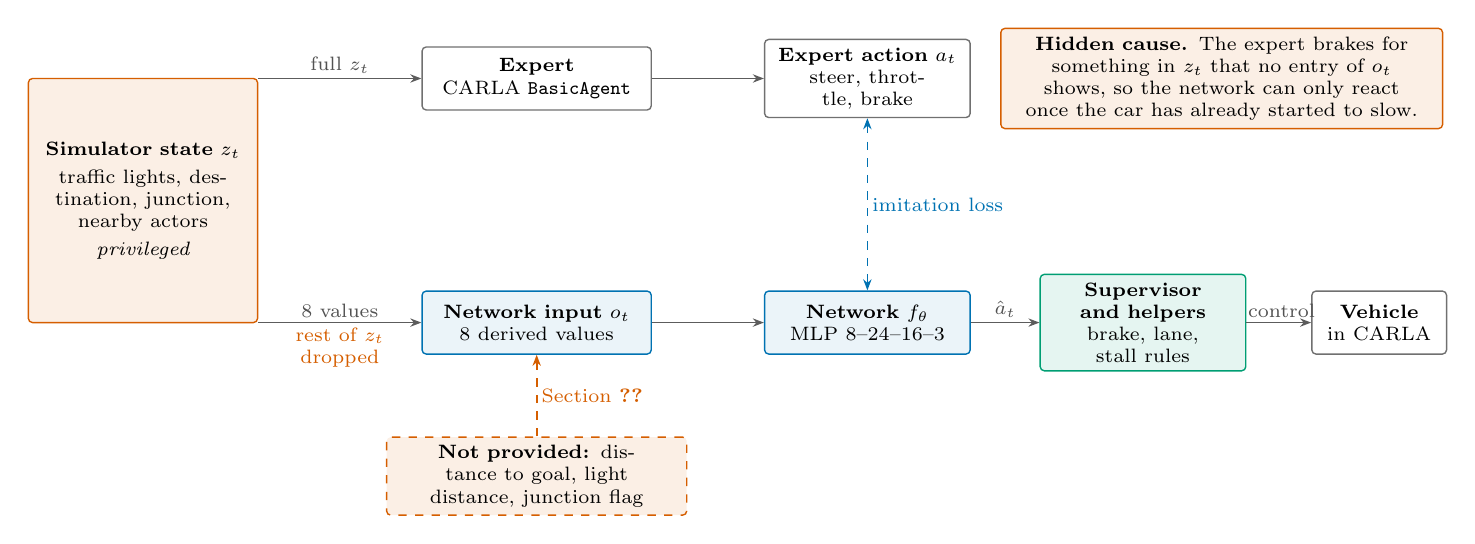
\begin{tikzpicture}[x=1cm,y=1cm]
% privileged simulator state
\node[hid, text width=2.7cm, minimum height=3.1cm] (sim) at (-0.4,0)
  {\textbf{Simulator state} $z_t$\\[2pt] traffic lights, destination,
   junction, nearby actors\\[2pt]\itshape privileged};
% top row: the expert
\node[box, text width=2.7cm] (exp) at (4.6,1.55)
  {\textbf{Expert}\\ CARLA \texttt{BasicAgent}};
\node[box, text width=2.4cm] (act) at (8.8,1.55)
  {\textbf{Expert action} $a_t$\\ steer, throttle, brake};
% bottom row: the learner and what surrounds it
\node[obs, text width=2.7cm] (obs) at (4.6,-1.55)
  {\textbf{Network input} $o_t$\\ 8 derived values};
\node[obs, text width=2.4cm] (net) at (8.8,-1.55)
  {\textbf{Network} $f_\theta$\\ MLP 8--24--16--3};
\node[help, text width=2.4cm] (hlp) at (12.3,-1.55)
  {\textbf{Supervisor and helpers}\\ brake, lane, stall rules};
\node[box, text width=1.5cm] (car) at (15.3,-1.55)
  {\textbf{Vehicle}\\ in CARLA};
% data flow
\draw[flow] (sim.east |- exp) -- node[lbl,above] {full $z_t$} (exp.west);
\draw[flow] (sim.east |- obs) -- node[lbl,above] {8 values}
  node[lbl,below,text=cHid] {rest of $z_t$\\dropped} (obs.west);
\draw[flow] (exp) -- (act);
\draw[flow] (obs) -- (net);
\draw[flow] (net) -- node[lbl,above] {$\hat a_t$} (hlp);
\draw[flow] (hlp) -- node[lbl,above,xshift=1pt] {control} (car);
% imitation loss
\draw[{Stealth[length=4pt]}-{Stealth[length=4pt]}, dashed, line width=0.6pt,
      draw=cObs] (act) -- node[lbl,right,text=cObs] {imitation loss} (net);
% what is dropped
% candidate inputs that repair the gap
\node[hid, dashed, text width=3.6cm] (cand) at (4.6,-3.5)
  {\textbf{Not provided:} distance to goal, light distance, junction flag};
\draw[flow, draw=cHid, dashed] (cand) -- node[lbl,right,text=cHid] {Section~\ref{sec:repair}} (obs);
% hidden cause call-out
\node[hid, text width=5.4cm, minimum height=1.25cm] (callout) at (13.3,1.55)
  {\textbf{Hidden cause.} The expert brakes for something in $z_t$ that no
   entry of $o_t$ shows, so the network can only react once the car has
   already started to slow.};
\end{tikzpicture}
\caption{System overview. The expert acts on the full simulator state
$z_t$; the network sees only eight derived values $o_t$ and is trained to
copy the expert's action. Anything in $z_t$ that never reaches $o_t$ is a
potential hidden cause (orange). The network output then passes through a
supervisor and helper rules before it reaches the car; Section~\ref{sec:shield}
measures how much those rules contribute.}
\label{fig:overview}
\end{figure*}

% =====================================================================
\section{Related Work}

\textbf{Limits of behaviour cloning.} Codevilla \textit{et
al.}~\cite{limits} showed that cloned driving policies fail in ways
that average error does not reveal, including inertia and
over-reliance on the expert's most common action. DAgger~\cite{dagger}
addresses distribution shift by letting the learner drive and querying
the expert. Neither asks whether the expert's cause is in the input.

\textbf{Causal confusion and copycat behaviour.} De Haan \textit{et
al.}~\cite{causalconf} showed that more information can make cloning
worse when the learner latches onto inputs that correlate with, but
do not cause, the expert's action. Wen \textit{et al.}~\cite{copycat}
showed that a learner given past actions or observations may simply
copy the previous action. Our setting is the complementary case: the
cause is \emph{absent} from the input. We also provide a measurement
that can be applied to a recorded dataset without training.

\textbf{Privileged experts.} Learning by Cheating~\cite{lbc} and
Roach~\cite{roach} train a privileged agent first and distil it into a
sensor-based policy. A privileged teacher is useful, but any gap
between what the teacher and student see is a source of hidden causes.
Our audit can be applied to the teacher--student pair.

\textbf{Shielding.} Safety shields~\cite{shield} filter actions so that
a specification is never violated. Safe RL surveys~\cite{safe} discuss
performance under such constraints. We ask a narrower evaluation
question: how much of a measured success comes from the shield?

% =====================================================================
\section{Problem Setting}

A dataset $\mathcal{D}=\{(o_t,a_t)\}_{t=1}^{N}$ records the inputs
$o_t\in\mathbb{R}^{d}$ and expert action $a_t=(s_t,u_t,b_t)$ (steering,
accelerator, brake). The expert additionally has access to a
privileged state $z_t$ (traffic lights, destination, junction, nearby
actors) that is available in the simulator but is not part of $o_t$.
The learner is trained to predict $a_t$ from $o_t$ (or a short window
of past inputs).

We say the action is \emph{observable} from $o$ if there is a function
$f$ such that $a_t\approx f(o_{t-W:t})$. Hidden cause means that $a_t$
depends on part of $z_t$ that cannot be recovered from $o_{t-W:t}$.

% =====================================================================
\section{The Observability Audit}\label{sec:audit}

\subsection{Action events}

Averaged error is dominated by frames where nothing changes. We
therefore audit \emph{events}. A \emph{brake onset} occurs at step $t$
when the brake rises from below $0.5$ to at least $0.5$ while the car is
moving (speed above 1\,km/h). We define throttle-release and
steering-onset events the same way. In this paper we report brake
onsets, which are the safety-critical case.

\subsection{Warning and Unexplained Event Rate}

For each input $i$ we define a change threshold $\tau_i$ (for flags,
any toggle; for continuous inputs, a fixed fraction of the normalised
range). An input \emph{warns} of an onset at $t$ if it changes by more
than $\tau_i$ within a window of $W$ steps before $t$. An onset is
\emph{unexplained} if no input warns of it. With $E$ the set of onsets,
\begin{equation}
\mathrm{UER}=\frac{\left|\{e\in E:\ \text{no input warns of }e\}\right|}{|E|}.
\label{eq:uer}
\end{equation}
UER depends on $W$ and $\tau$, so we report it over a grid of both
(Section~\ref{sec:sens}) and use $W=1$\,s as the default.
Fig.~\ref{fig:audit} shows one explained and one unexplained onset.

\begin{figure*}[!t]
\centering
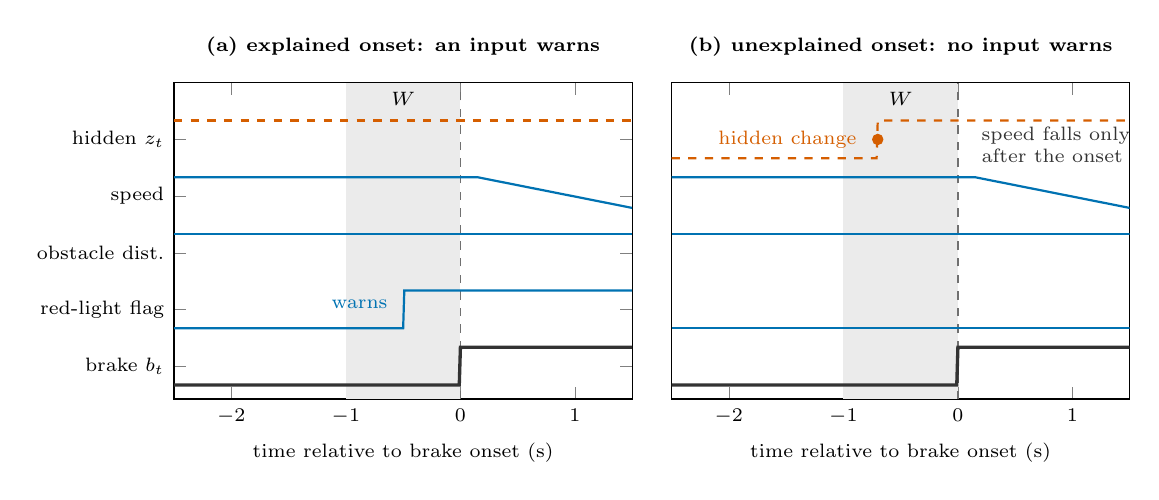
\begin{tikzpicture}
\begin{axis}[name=A, width=7.4cm, height=5.6cm, xmin=-2.5, xmax=1.5,
  ymin=-0.3, ymax=6.4, xlabel={time relative to brake onset (s)},
  ytick={0.4,1.6,2.8,4.0,5.2},
  yticklabels={brake $b_t$,red-light flag,obstacle dist.,speed,hidden $z_t$},
  xtick={-2,-1,0,1}, title={(a) explained onset: an input warns}]
  \fill[black!8] (axis cs:-1,-0.3) rectangle (axis cs:0,6.4);
  \node[font=\scriptsize] at (axis cs:-0.5,6.05) {$W$};
  \draw[dashed, cInk!70] (axis cs:0,-0.3) -- (axis cs:0,6.4);
  \addplot[cInk, very thick] coordinates {(-2.5,0)(-0.01,0)(0,0.8)(1.5,0.8)};
  \addplot[cObs, thick] coordinates {(-2.5,1.2)(-0.5,1.2)(-0.49,2.0)(1.5,2.0)};
  \addplot[cObs, thick] coordinates {(-2.5,3.2)(1.5,3.2)};
  \addplot[cObs, thick] coordinates {(-2.5,4.4)(0.15,4.4)(1.5,3.75)};
  \addplot[cHid, thick, dashed] coordinates {(-2.5,5.6)(1.5,5.6)};
  \node[font=\scriptsize, text=cObs, anchor=east] at (axis cs:-0.55,1.7) {warns};
\end{axis}
\begin{axis}[at={($(A.east)+(0.5cm,0)$)}, anchor=west, width=7.4cm, height=5.6cm,
  xmin=-2.5, xmax=1.5, ymin=-0.3, ymax=6.4,
  xlabel={time relative to brake onset (s)}, ytick=\empty, xtick={-2,-1,0,1},
  title={(b) unexplained onset: no input warns}]
  \fill[black!8] (axis cs:-1,-0.3) rectangle (axis cs:0,6.4);
  \node[font=\scriptsize] at (axis cs:-0.5,6.05) {$W$};
  \draw[dashed, cInk!70] (axis cs:0,-0.3) -- (axis cs:0,6.4);
  \addplot[cInk, very thick] coordinates {(-2.5,0)(-0.01,0)(0,0.8)(1.5,0.8)};
  \addplot[cObs, thick] coordinates {(-2.5,1.2)(1.5,1.2)};
  \addplot[cObs, thick] coordinates {(-2.5,3.2)(1.5,3.2)};
  \addplot[cObs, thick] coordinates {(-2.5,4.4)(0.15,4.4)(1.5,3.75)};
  \addplot[cHid, thick, dashed] coordinates {(-2.5,4.8)(-0.71,4.8)(-0.7,5.6)(1.5,5.6)};
  \addplot[only marks, mark=*, mark size=1.8pt, cHid] coordinates {(-0.7,5.2)};
  \node[font=\scriptsize, text=cHid, anchor=east] at (axis cs:-0.8,5.2) {hidden change};
  \node[font=\scriptsize, text=cInk, anchor=south west, align=left] at (axis cs:0.12,4.5)
    {speed falls only\\after the onset};
\end{axis}
\end{tikzpicture}
\caption{Schematic of the audit on a single brake onset (not recorded
data). Shaded: the window $W$ before the onset. In (a) the red-light flag
toggles inside $W$, so an input warns of the onset. In (b) the only
change inside $W$ is in a variable the network does not receive (orange,
dashed); the inputs change only after the car starts to slow, so the
onset counts toward UER.}
\label{fig:audit}
\end{figure*}

\subsection{Predictive lead time}

UER is a coarse count. As a finer test we train a small held out
classifier that predicts whether a brake onset will occur within
the next $k$ steps from the input window, and measure the largest $k$
at which it stays above a fixed score. A short lead time means that the
inputs carry information about the stop only after it has begun.
Training and evaluation use a split by whole routes to avoid leakage
between adjacent frames.

\subsection{Observability gap}

If privileged candidate features $c_t\subset z_t$ are available we
compare the held out error of a predictor using $o_t$ with one using
$(o_t,c_t)$ on onset windows. The difference is the \emph{observability
gap} $\Delta$ for that candidate. A candidate with a large $\Delta$
is a plausible missing cause. A candidate with $\Delta\approx0$ is not.

% =====================================================================
\section{Preliminary Evidence from an Existing Dataset}\label{sec:prelim}

All numbers in this section were measured on data recorded for our
earlier imitation learning project.

\subsection{Data and network}

\texttt{BasicAgent} drove 12 complete routes on \texttt{Town02\_Opt},
giving 19{,}750 samples, split by whole route into 8 training (13{,}052
samples), 2 validation (2{,}973) and 2 test (3{,}725) routes. The
network is a multilayer perceptron with eight inputs, hidden layers of
24 and 16 units with $\tanh$, and three outputs (667 trainable
parameters). The inputs are lane
error, heading error, speed, target speed, front obstacle distance, red
light flag, curvature and a stopped flag.

\subsection{Average error is low}

Table~\ref{tab:base} and Fig.~\ref{fig:prelim}(b) show held out error on
the two test routes.

\begin{table}[htbp]
\caption{Held out error of the baseline network}
\label{tab:base}
\centering\footnotesize
\begin{tabular}{@{}lr@{}}
\toprule
Measure & Value \\
\midrule
Test mean squared error          & 0.0157 \\
Steering mean absolute error     & 0.0147 \\
Accelerator mean absolute error  & 0.0806 \\
Brake mean absolute error        & 0.0664 \\
\bottomrule
\end{tabular}
\end{table}

\subsection{But stops start late and have no visible cause}

On the test routes the network predicted less than half brake in 3.8\%
of frames where the expert braked fully, all within 0.7\,s of a stop
starting, and braked hard when the expert did not in 2.1\% of frames.
Across the whole dataset the expert started braking 40 times while
moving. The red light flag was on within one second of only 5 of them,
and in 35 of the 40 onsets no input warned of the stop. Under
Eq.~\eqref{eq:uer} with $W=1$\,s this gives a preliminary
$\mathrm{UER}=35/40=87.5\%$ (Fig.~\ref{fig:prelim}(c)). With only 40
events the uncertainty matters: the 95\% Wilson
interval~\cite{wilson,brown} for 35 of 40 is 73.9--94.5\%, so even the
low end of the interval leaves most onsets unexplained.
The recordings also contain no other
vehicle: the obstacle input is at its ``nothing ahead'' value in every
frame, and the car is stopped in 44.6\% of frames.

\textbf{What this does and does not show.} It shows that the eight
inputs do not announce most stops. It does \emph{not} yet show what
causes them. The dataset has no vehicles, so the cause is not another
car. Section~\ref{sec:repair} describes how we find out.

\begin{figure*}[!t]
\centering
\begin{minipage}[t]{0.31\textwidth}
\centering
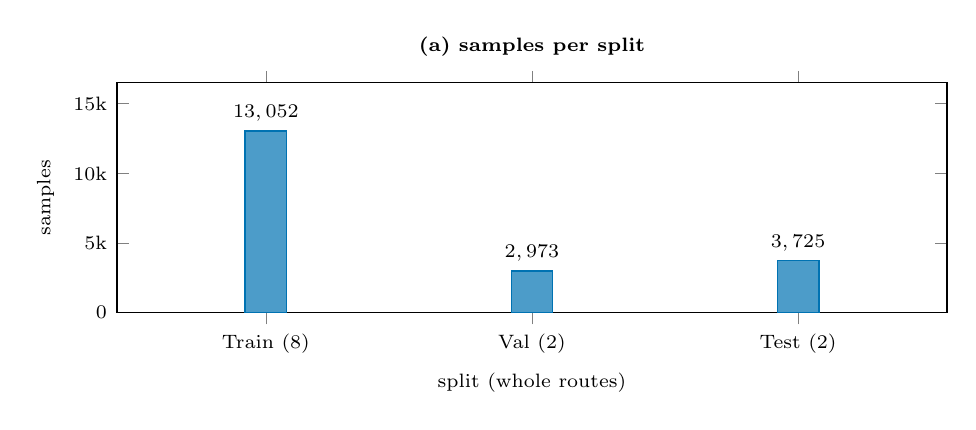
\begin{tikzpicture}[baseline=(current bounding box.north)]
\begin{axis}[ybar, width=\linewidth, height=4.5cm, bar width=15pt,
  symbolic x coords={Train,Val,Test}, xtick=data,
  xticklabels={Train (8),Val (2),Test (2)},
  ymin=0, ymax=16500, enlarge x limits=0.28,
  xlabel={split (whole routes)},
  ylabel={samples}, ytick={0,5000,10000,15000},
  yticklabels={0,5k,10k,15k}, scaled y ticks=false,
  title={(a) samples per split},
  nodes near coords, nodes near coords align={vertical},
  every node near coord/.append style={font=\scriptsize,
    /pgf/number format/fixed, /pgf/number format/precision=0,
    /pgf/number format/1000 sep={{,}}}]
  \addplot[fill=cObs!70, draw=cObs] coordinates {(Train,13052)(Val,2973)(Test,3725)};
\end{axis}
\end{tikzpicture}
\end{minipage}\hfill
\begin{minipage}[t]{0.31\textwidth}
\centering
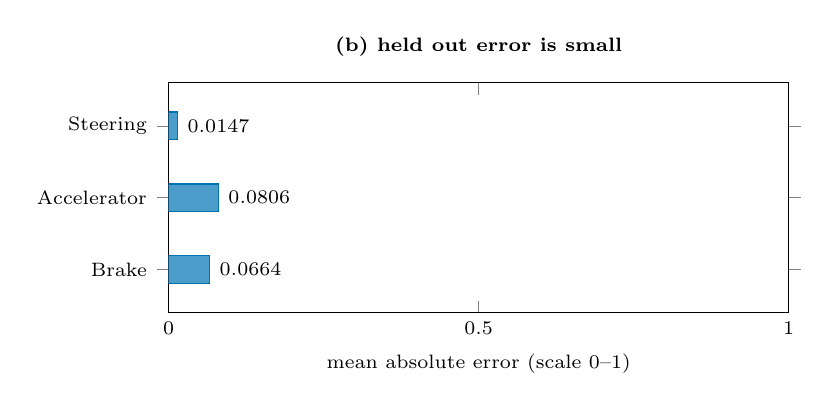
\begin{tikzpicture}[baseline=(current bounding box.north)]
\begin{axis}[xbar, width=0.78\linewidth, height=4.5cm, bar width=10pt,
  symbolic y coords={Brake,Accelerator,Steering}, ytick=data,
  xmin=0, xmax=1, enlarge y limits=0.3,
  xlabel={mean absolute error (scale 0--1)},
  xtick={0,0.5,1},
  title={(b) held out error is small},
  nodes near coords, nodes near coords align={horizontal},
  every node near coord/.append style={font=\scriptsize,
    /pgf/number format/fixed, /pgf/number format/precision=4}]
  \addplot[fill=cObs!70, draw=cObs] coordinates {(0.0664,Brake)(0.0806,Accelerator)(0.0147,Steering)};
\end{axis}
\end{tikzpicture}
\end{minipage}\hfill
\begin{minipage}[t]{0.31\textwidth}
\centering
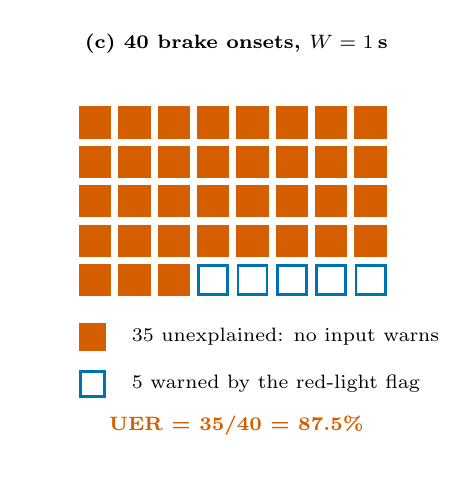
\begin{tikzpicture}[x=0.5cm,y=0.5cm,baseline=(current bounding box.north)]
\useasboundingbox (-1.3,-8.7) rectangle (9.3,2.0);
\node[font=\scriptsize\bfseries] at (4,1.6) {(c) 40 brake onsets, $W=1$\,s};
\foreach \i in {0,...,39}{
  \pgfmathtruncatemacro{\r}{int(\i/8)}
  \pgfmathtruncatemacro{\c}{mod(\i,8)}
  \ifnum\i<35
    \fill[cHid] (\c,-\r) rectangle ++(0.82,-0.82);
  \else
    \draw[cObs, fill=white, line width=1pt] (\c+0.04,-\r-0.04) rectangle ++(0.74,-0.74);
  \fi
}
\fill[cHid] (0,-5.5) rectangle ++(0.7,-0.7);
\node[font=\scriptsize, anchor=west] at (1.1,-5.85) {35 unexplained: no input warns};
\draw[cObs, fill=white, line width=1pt] (0.04,-6.74) rectangle ++(0.62,-0.62);
\node[font=\scriptsize, anchor=west] at (1.1,-7.05) {5 warned by the red-light flag};
\node[font=\scriptsize\bfseries, text=cHid] at (4,-8.1) {UER = 35/40 = 87.5\%};
\end{tikzpicture}
\end{minipage}
\caption{Measured on the 12-route dataset. (a) Samples in each split,
with the number of whole routes in brackets. (b) Mean absolute error on
the two test routes; every output is close to zero on a 0--1 scale. (c) The 40 brake
onsets: 35 have no warning in any of the eight inputs (filled), only 5 are
announced by the red light flag (outlined), giving
$\mathrm{UER}=87.5\%$, 95\% Wilson interval 73.9--94.5\%.}
\label{fig:prelim}
\end{figure*}

% =====================================================================
\section{Cause Attribution and Repair}\label{sec:repair}

\subsection{Logging the privileged state}

We replay or re-record the 12 routes and log, at every step, the expert's
privileged variables $z_t$: traffic light state and distance to the
nearest light the expert considers, distance remaining to the
destination, whether the car is entering a junction, the planner's road
option at the next waypoint, speed limit, and the nearest actor
distance and speed. For each of the 40 onsets we label the variable that
changed first.

\subsection{Hypotheses}

We have not determined the cause. Candidate explanations that fit a
dataset with no other vehicles are:
\begin{itemize}
\setlength{\itemsep}{1pt}
\item \textbf{H1: approach to the route end.} The expert slows to stop
at the destination, which is not an input.
\item \textbf{H2: earlier traffic light detection.} The expert reacts to
a light at a longer range than the network's red light flag covers.
\item \textbf{H3: junction or road option.} The expert slows for a turn
announced by the planner's road option, which the controller ignores.
\item \textbf{H4: other or mixed.}
\end{itemize}
The audit is useful whichever hypothesis holds. It tells us which one.
Fig.~\ref{fig:protocol} summarises the protocol.

\begin{figure*}[!t]
\centering
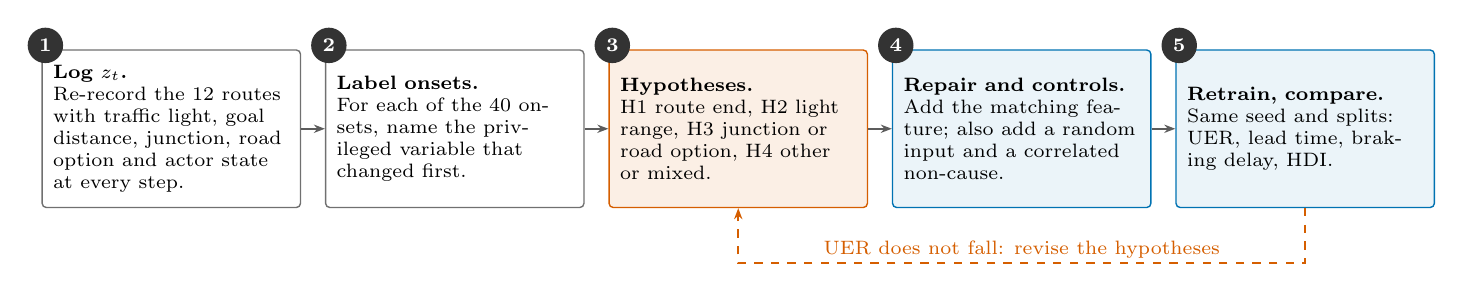
\begin{tikzpicture}[x=1cm,y=1cm]
\tikzset{pbox/.style={text width=3.0cm, minimum height=2.0cm, align=left,
                      inner sep=4pt},
         num/.style={circle, fill=cInk, text=white, font=\scriptsize\bfseries,
                     inner sep=1.5pt, minimum size=0.45cm}}
\node[box, pbox] (s1) at (0,0)
  {\textbf{Log $z_t$.}\\ Re-record the 12 routes with traffic light, goal
   distance, junction, road option and actor state at every step.};
\node[box, pbox] (s2) at (3.6,0)
  {\textbf{Label onsets.}\\ For each of the 40 onsets, name the privileged
   variable that changed first.};
\node[hid, pbox] (s3) at (7.2,0)
  {\textbf{Hypotheses.}\\ H1 route end, H2 light range, H3 junction or road
   option, H4 other or mixed.};
\node[obs, pbox] (s4) at (10.8,0)
  {\textbf{Repair and controls.}\\ Add the matching feature; also add a
   random input and a correlated non-cause.};
\node[obs, pbox] (s5) at (14.4,0)
  {\textbf{Retrain, compare.}\\ Same seed and splits: UER, lead time,
   braking delay, HDI.};
\foreach \a/\b in {s1/s2,s2/s3,s3/s4,s4/s5}
  \draw[flow] (\a.east) -- (\b.west);
\foreach \s/\n in {s1/1,s2/2,s3/3,s4/4,s5/5}
  \node[num] at ($(\s.north west)+(0.05,0.05)$) {\n};
\draw[flow, dashed, draw=cHid] (s5.south) -- ++(0,-0.7) -|
  node[lbl, pos=0.25, above, text=cHid] {UER does not fall: revise the hypotheses} (s3.south);
\end{tikzpicture}
\caption{Cause attribution and repair protocol. Controls (step 4) check
that UER does not fall merely because an input was added; the feedback
arrow marks the case where the first hypothesis is wrong.}
\label{fig:protocol}
\end{figure*}

\subsection{Repair experiment}

For each supported hypothesis we add the matching feature (for example,
distance to destination, distance to next light and its state, a
junction flag) to the input contract, retrain with the same seed and
splits, and measure:
\begin{enumerate}
\setlength{\itemsep}{1pt}
\item UER, expected to fall if the feature is the missing cause;
\item predictive lead time and observability gap $\Delta$;
\item late braking, the delay between the expert's onset and the
network's brake crossing 0.5.
\end{enumerate}
As controls we add (i) a random input and (ii) a feature that
correlates with stopping but is not its cause, in order to check that
UER does not fall simply because an input was added.

\begin{table}[htbp]
\caption{Repair experiment: input sets compared}
\label{tab:repair}
\centering\footnotesize
\begin{tabular}{@{}lL{4.2cm}@{}}
\toprule
Input set & Purpose \\
\midrule
Baseline (8 inputs)        & reference; UER = 87.5\% \\
+ distance to destination  & tests H1 \\
+ light state and distance & tests H2 \\
+ junction flag            & tests H3 \\
+ random input             & control: no causal content \\
+ correlated non-cause     & control: correlates with stopping \\
\bottomrule
\end{tabular}
\end{table}

\subsection{Sensitivity}\label{sec:sens}

We report UER over $W\in\{0.5,1,2\}$\,s and several values of $\tau$,
and with onset definitions at brake thresholds of $0.3$, $0.5$ and
$0.7$, to show that conclusions do not depend on one choice.

% =====================================================================
\section{Helper Attribution}\label{sec:shield}

Our driving stack places a safety supervisor and several helper rules
between the network and the car (Table~\ref{tab:helpers}). The
supervisor applies full brake for conditions such as a collision, an
obstacle closer than 7\,m or a red light, and a stall recovery adds a
small throttle when the car sits still. The stall recovery exists because
the baseline can hold the brake at a standstill on a clear road, which
the code documents as a known failure mode of the policy; a network that
cannot restart on its own would show a high dependence on helpers by
construction. We evaluate three configurations (Fig.~\ref{fig:helpers})
on routes the network was not trained on, using the same seeds:
\begin{enumerate}
\setlength{\itemsep}{1pt}
\item \textbf{Raw:} network output only, converted to a vehicle command
with no other rule.
\item \textbf{Supervised:} network plus supervisor.
\item \textbf{Full:} network plus supervisor plus all helpers.
\end{enumerate}
For each we record route completion $C$, collisions and lane departures
per km, and the \emph{override rate}, the fraction of steps on which the
applied control differs from the network output (any rule in
Table~\ref{tab:helpers} counts). We define the Helper
Dependence Index
\begin{equation}
\mathrm{HDI}=\frac{C_{\text{full}}-C_{\text{raw}}}{C_{\text{full}}},
\end{equation}
which is near 0 when the network completes routes on its own and near 1
when the helpers do nearly all the work. We report HDI before and after
the repair in Section~\ref{sec:repair}, which tests whether giving the
network the missing input reduces its dependence on the helpers.

The brake deadband in Table~\ref{tab:helpers} deserves attention. It
zeroes any network brake output below 0.45, close to the 0.5 level that
defines a brake onset (Section~\ref{sec:audit}), so a weak or late
network brake can be removed before it reaches the supervisor. Counting
it in the override rate keeps this effect visible.

\begin{figure}[!t]
\centering
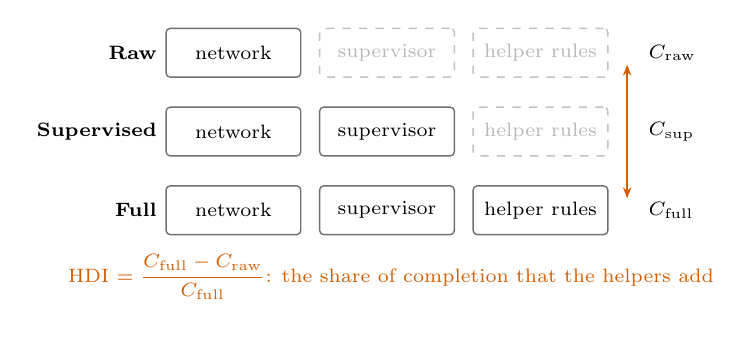
\begin{tikzpicture}[x=1cm,y=1cm]
\tikzset{chip/.style={box, text width=1.5cm, minimum height=0.62cm},
         off/.style={chip, draw=cInk!30, text=cInk!35, fill=none, dashed}}
\node[anchor=east, font=\scriptsize\bfseries] at (1.35,1.0) {Raw};
\node[anchor=east, font=\scriptsize\bfseries] at (1.35,0.0) {Supervised};
\node[anchor=east, font=\scriptsize\bfseries] at (1.35,-1.0) {Full};
% Raw
\node[obs, chip] at (2.2,1.0) {network};
\node[off] at (4.15,1.0) {supervisor};
\node[off] at (6.1,1.0) {helper rules};
% Supervised
\node[obs, chip] at (2.2,0.0) {network};
\node[help, chip] at (4.15,0.0) {supervisor};
\node[off] at (6.1,0.0) {helper rules};
% Full
\node[obs, chip] at (2.2,-1.0) {network};
\node[help, chip] at (4.15,-1.0) {supervisor};
\node[help, chip] at (6.1,-1.0) {helper rules};
% completion labels
\node[anchor=west, font=\scriptsize] at (7.35,1.0) {$C_{\text{raw}}$};
\node[anchor=west, font=\scriptsize] at (7.35,0.0) {$C_{\text{sup}}$};
\node[anchor=west, font=\scriptsize] at (7.35,-1.0) {$C_{\text{full}}$};
\draw[{Stealth[length=4pt]}-{Stealth[length=4pt]}, line width=0.6pt, draw=cHid]
  (7.2,0.85) -- (7.2,-0.85);
\node[align=center, font=\scriptsize, text=cHid] at (4.2,-1.85)
  {HDI $=\dfrac{C_{\text{full}}-C_{\text{raw}}}{C_{\text{full}}}$:
   the share of completion that the helpers add};
\end{tikzpicture}
\caption{The three evaluation configurations. Solid boxes are active,
dashed grey boxes are switched off. For each configuration we measure
route completion, override rate, and collisions and lane departures per
km; HDI compares route completion between the outer two rows.}
\label{fig:helpers}
\end{figure}

\begin{table}[htbp]
\caption{Rules between the network and the car (library defaults; entry
points may override them)}
\label{tab:helpers}
\centering\scriptsize
\setlength{\tabcolsep}{3pt}
\begin{tabular}{@{}L{1.45cm}L{2.75cm}L{3.55cm}@{}}
\toprule
Rule & Fires when & Effect \\
\midrule
Supervisor & collision, obstacle $<7$\,m, red light, lane error
$>2$\,m, speed $>50$\,km/h, command older than 0.25\,s, sensor timeout
& full brake (hand brake on collision) \\\addlinespace[2pt]
Brake deadband & network brake $<0.45$, no emergency stop & brake set to 0 \\\addlinespace[2pt]
Lane assist & lane error $\le2$\,m, no red light, obstacle $\ge7$\,m
& steering nudged toward lane centre by at most 0.16; target speed
lowered when displaced or turning \\\addlinespace[2pt]
Stall recovery & standstill for 2\,s (5\,s if the network brakes), road
clear & throttle up to 0.35 and network brake released; ends at 85\% of
target speed \\\addlinespace[2pt]
Speed limiter & speed near or above target & throttle eased within
3\,km/h of target; brake up to 0.5 when over by more than 1\,km/h \\
\bottomrule
\end{tabular}
\end{table}

% =====================================================================
\section{Threats to Validity}

\textbf{One town, one expert.} All current data come from one town and
one rule-based expert. We plan to repeat the audit on at least one more
map. \textbf{Small event count.} Forty onsets is small: the 95\% Wilson
interval for UER is 73.9--94.5\% (Fig.~\ref{fig:ci}). If the observed
rate holds, about 170 onsets would narrow the interval to $\pm5$ points
and about 670 to $\pm2.5$ points, so we will re-record more routes and
report intervals throughout. \textbf{Threshold
dependence.} UER depends on $W$ and $\tau$; Section~\ref{sec:sens}
reports the spread. \textbf{Correlation is not cause.} A feature that
lowers UER may merely correlate with the true cause; the control
features are intended to catch this. \textbf{Simulation only.}
Conclusions apply to CARLA and a rule-based expert.

\begin{figure}[!t]
\centering
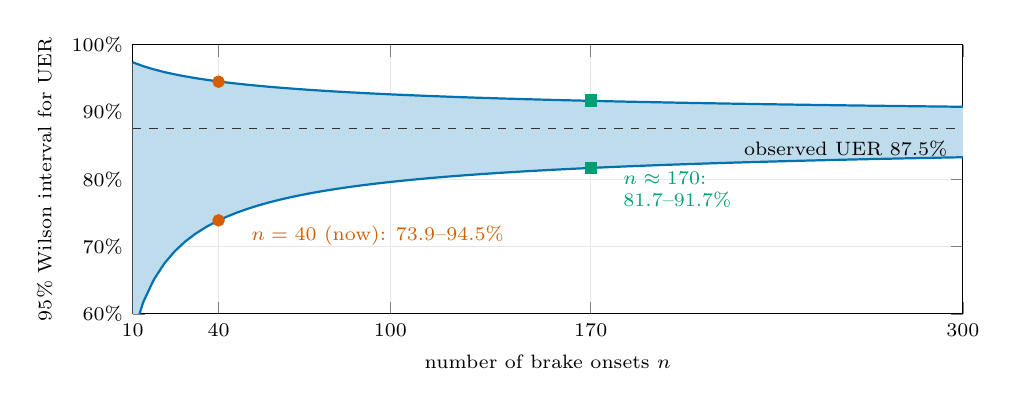
\begin{tikzpicture}
\begin{axis}[width=\columnwidth, height=5.0cm, xmin=10, xmax=300,
  ymin=0.6, ymax=1.0, xlabel={number of brake onsets $n$},
  ylabel={95\% Wilson interval for UER},
  ytick={0.6,0.7,0.8,0.9,1.0}, yticklabels={60\%,70\%,80\%,90\%,100\%},
  xtick={10,40,100,170,300}, grid=major, grid style={cInk!12}]
  \addplot[name path=lo, draw=none, domain=10:300, samples=80]
    {(0.875+1.9208/x-1.96*sqrt(0.109375/x+0.9604/(x*x)))/(1+3.8416/x)};
  \addplot[name path=hi, draw=none, domain=10:300, samples=80]
    {(0.875+1.9208/x+1.96*sqrt(0.109375/x+0.9604/(x*x)))/(1+3.8416/x)};
  \addplot[cObs!25] fill between[of=lo and hi];
  \addplot[cObs, thick, domain=10:300, samples=80]
    {(0.875+1.9208/x-1.96*sqrt(0.109375/x+0.9604/(x*x)))/(1+3.8416/x)};
  \addplot[cObs, thick, domain=10:300, samples=80]
    {(0.875+1.9208/x+1.96*sqrt(0.109375/x+0.9604/(x*x)))/(1+3.8416/x)};
  \addplot[cInk, dashed, domain=10:300] {0.875};
  \addplot[only marks, mark=*, mark size=2pt, cHid] coordinates {(40,0.739)(40,0.945)};
  \addplot[only marks, mark=square*, mark size=2pt, cHelp] coordinates {(170,0.817)(170,0.917)};
  \node[font=\scriptsize, text=cHid, anchor=north west, align=left] at (axis cs:48,0.745)
    {$n=40$ (now): 73.9--94.5\%};
  \node[font=\scriptsize, text=cHelp, anchor=north west, align=left] at (axis cs:178,0.825)
    {$n\approx170$:\\81.7--91.7\%};
  \node[font=\scriptsize, anchor=north east] at (axis cs:298,0.871) {observed UER 87.5\%};
\end{axis}
\end{tikzpicture}
\caption{How the uncertainty in UER shrinks with the number of onsets,
assuming the observed rate of 87.5\% stays the same (a planning
calculation, not new data). The interval at $n=40$ is the one
reported in Section~\ref{sec:prelim}.}
\label{fig:ci}
\end{figure}

% =====================================================================
\section{Plan of Work}

Table~\ref{tab:plan} orders the work so that each phase ends in a result
that can be checked on its own.

\begin{table}[htbp]
\caption{Phases, each ending in a usable result}
\label{tab:plan}
\centering\scriptsize
\setlength{\tabcolsep}{3pt}
\begin{tabular}{@{}lL{6.9cm}@{}}
\toprule
Phase & Goal and exit check \\
\midrule
1 & Implement event detection and UER on the existing 12 routes.
\emph{Exit:} UER reproduced for a grid of $W$ and $\tau$. \\
2 & Re-record with privileged logging and label the cause of each onset.
\emph{Exit:} every onset has a label. \\
3 & Add features, retrain, and run the controls.
\emph{Exit:} Table~\ref{tab:repair} configurations evaluated. \\
4 & Raw, supervised and full evaluation on unseen routes.
\emph{Exit:} Fig.~\ref{fig:helpers} configurations evaluated. \\
5 & Second town, confidence intervals, write up. \\
\bottomrule
\end{tabular}
\end{table}

% =====================================================================
\section{Conclusion}

A low prediction error can hide the fact that the expert acts for reasons
the learner cannot see. We proposed an audit that counts unexplained
action events before training, a procedure to find and repair the missing
cause, and an evaluation that separates the network's skill from that of
the safety helpers around it. Preliminary measurements on our existing
dataset, with 35 of 40 brake onsets unexplained (95\% Wilson interval
73.9--94.5\%), motivate the work. The
cause attribution, repair and helper-attribution protocols define the
experiments that complete the study.

% =====================================================================
\begin{thebibliography}{99}
\footnotesize
\setlength{\itemsep}{0pt}\setlength{\parsep}{0pt}

\bibitem{bojarski} M. Bojarski \textit{et al.}, ``End to End Learning
for Self-Driving Cars,'' NVIDIA, 2016. arXiv:1604.07316.

\bibitem{carla} A. Dosovitskiy \textit{et al.}, ``CARLA: An Open Urban
Driving Simulator,'' \emph{CoRL}, 2017. arXiv:1711.03938.

\bibitem{limits} F. Codevilla \textit{et al.}, ``Exploring the
Limitations of Behavior Cloning for Autonomous Driving,'' \emph{ICCV},
2019.

\bibitem{dagger} S. Ross, G. Gordon, and J. A. Bagnell, ``A Reduction of
Imitation Learning and Structured Prediction to No-Regret Online
Learning,'' \emph{AISTATS}, 2011. arXiv:1011.0686.

\bibitem{causalconf} P. de Haan, D. Jayaraman, and S. Levine, ``Causal
Confusion in Imitation Learning,'' \emph{NeurIPS}, 2019.

\bibitem{copycat} C. Wen, J. Lin, T. Darrell, D. Jayaraman, and Y. Gao,
``Fighting Copycat Agents in Behavioral Cloning from Observation
Histories,'' \emph{NeurIPS}, 2020.

\bibitem{lbc} D. Chen \textit{et al.}, ``Learning by Cheating,''
\emph{CoRL}, 2019. arXiv:1912.12294.

\bibitem{roach} Z. Zhang, A. Liniger, D. Dai, F. Yu, and L. Van Gool,
``End-to-End Urban Driving by Imitating a Reinforcement Learning
Coach,'' \emph{ICCV}, 2021.

\bibitem{shield} M. Alshiekh \textit{et al.}, ``Safe Reinforcement
Learning via Shielding,'' \emph{AAAI}, 2018.

\bibitem{safe} J. Garc\'{\i}a and F. Fern\'andez, ``A Comprehensive
Survey on Safe Reinforcement Learning,'' \emph{JMLR}, vol.~16, 2015.

\bibitem{wilson} E. B. Wilson, ``Probable inference, the law of
succession, and statistical inference,'' \emph{J. Amer. Statist. Assoc.},
vol.~22, no.~158, pp.~209--212, 1927.

\bibitem{brown} L. D. Brown, T. T. Cai, and A. DasGupta, ``Interval
estimation for a binomial proportion,'' \emph{Statist. Sci.}, vol.~16,
no.~2, pp.~101--133, 2001.

\end{thebibliography}

\end{document}
